\chapter{Results and Discussion}
\label{ch:results}

This chapter reports the main reconstruction result, the validation studies, and how sensing configuration governs reconstruction quality. The pipeline is: sensor placement $\to$ sensor measurements (here, DNS samples) $\to$ sensor-only physics training $\to$ continuous field reconstruction. Placement uses a low-cost LES in the main pipeline and is compared with two alternatives. The chapter proceeds from the headline result, field and spectral characterisation, and architectural ablation; through sensor count, placement, and noise studies; to a higher-Reynolds feasibility case, diagnostic boundaries, and inference cost.

\section{Main Result on $Re=10\,000$ Kolmogorov Flow}
\label{sec:main_result}

The main result uses the DNS-free LES-derived placement (one of the three placement strategies studied; \S\ref{sec:placement_analysis}): a one-head PI-CON readout, $1024$ physics-collocation points, and $K=100$ sensor locations selected from a long-horizon ($T_{\rm end}=50$~s) LES trajectory rather than DNS. Both the LES-pivot and DNS-pivot configurations are evaluated over the same $n=5$ random seeds at $20\,000$ training iterations, differing only in the sensor-placement source; Table~\ref{tab:main_metrics} therefore isolates placement quality.

\begin{table}[!htbp]
    \centering
    \caption{Main result and DNS-oracle placement reference at $Re=10\,000$, $K=100$, $n=5$ seeds, $20\,000$ iterations. Columns differ only in sensor-placement source. Values: mean $\pm$ sample standard deviation over seeds $\{42, 1, 2, 3, 4\}$. The KE, $u$, $v$, and $\omega$ errors are time-averaged over $t\in[0,T]$ (KE is MAPE). Relative-error metrics are percentages; divergence ratio $= \Vert\nabla\!\cdot\!\mathbf{u}\Vert_2 / \Vert\nabla\mathbf{u}\Vert_F^{\rm DNS}$.}
    \label{tab:main_metrics}
    \footnotesize
    \setlength{\tabcolsep}{3pt}
    \begin{tabularx}{\textwidth}{
        >{\raggedright\arraybackslash}p{3.2cm}
        >{\centering\arraybackslash}X
        >{\centering\arraybackslash}X
    }
    \toprule
    \textbf{Metric} & \textbf{LES placement} & \textbf{DNS-oracle placement} \\
    & \textbf{LES sensors ($n=5$, 20k iter)} & \textbf{DNS sensors ($n=5$, 20k iter)} \\
    \midrule
    Sensor placement source & LES $T=50$ & DNS oracle \\
    Physics collocation points & $1024$ & $1024$ \\
    KE MAPE & $5.71 \pm 0.11\%$ & $\mathbf{4.68 \pm 0.06\%}$ \\
    $u$ rel-$L_2$ & $\mathbf{13.65 \pm 0.06\%}$ & $15.34 \pm 0.06\%$ \\
    $v$ rel-$L_2$ & $\mathbf{17.52 \pm 0.10\%}$ & $18.10 \pm 0.03\%$ \\
    $\omega$ rel-$L_2$ & $\mathbf{41.79 \pm 0.12\%}$ & $42.41 \pm 0.12\%$ \\
    Divergence ratio & $0.39 \pm 0.006\%$ & $0.36 \pm 0.004\%$ \\
    $k_f$ amplitude ratio & $0.991 \pm 0.005$ & $0.986 \pm 0.005$ \\
    \bottomrule
    \end{tabularx}
\end{table}

\paragraph{Comparison boundary.}
The closest published sensor-only-with-physics comparison, Mo and Magri~\cite{Mo2025PRF}, addresses the same regime with a fixed-grid convolutional backbone; supervision-regime and architectural caveats are discussed in \S\ref{sec:literature}. Classical interpolation and older development baselines are not used as Chapter~\ref{ch:results} evidence because their reported numbers were not regenerated under the final $20\,000$-iteration, $1024$-collocation PI-CON protocol.

\paragraph{Time-segment decomposition.}
Table~\ref{tab:time_local} reports early, mid, and late segment averages from the main pipeline, diagnosing when reconstruction is hardest without altering the baseline definition; the worst single-time KE MAPE is $29.96\%$, at $t = 0.10$~s.

\paragraph{Discussion.}
The main row in Table~\ref{tab:main_metrics} uses no DNS full field for sensor placement or training supervision; sensor values are the DNS stand-in sampled only at the $K$ positions. Against the DNS-oracle reference, placement shows an integral/pointwise trade-off: the oracle has lower KE error ($4.68\%$ vs $5.71\%$), while LES-derived placement has lower pointwise velocity error ($u$ rel-$L_2$ $13.65\%$ vs $15.34\%$, $v$ rel-$L_2$ $17.52\%$ vs $18.10\%$). All strategies remain within the $10\%$ target: random placement gives KE $7.95\%$, LES-derived placement $5.71\%$, and the non-deployable DNS oracle $4.68\%$. LES-derived placement is therefore adopted as the reference DNS-free configuration because it improves over random by $2.24$ KE percentage points and reduces placement-induced variance roughly sixfold (\S\ref{sec:placement_analysis}).

The divergence ratio of $0.39\%$ confirms the continuity constraint is active, matching the finite-difference floor of a DNS field band-limited to the reconstruction's resolved bandwidth (\S\ref{sec:sub_dns_div}; Fig.~\ref{fig:main_trajectories}, second panel). The energy-dominant low-wavenumber band (sensor-count Nyquist scale $k_{\max}^{\rm sensor}\approx 5.64$, carrying $\approx 99\%$ of kinetic energy at $t=5$; \S\ref{subsec:nyquist_scaling}) recovers to single-digit relative error (Fig.~\ref{fig:band_err}), within the $10\%$ engineering target of O1.

Error is largest over the first half-second, consistent with the difficulty of reconstructing the initial condition from sensor history alone, and declines steadily thereafter (Fig.~\ref{fig:main_trajectories}, first panel). The time-mean KE error in Table~\ref{tab:main_metrics} therefore aggregates a decaying transient rather than a stationary error level. The sensor-count sweep in \S\ref{subsec:nyquist_scaling} is single-seed, but uses the final PI-CON protocol and is interpreted only as a bandwidth trend.

\begin{figure}[!htbp]
    \centering
    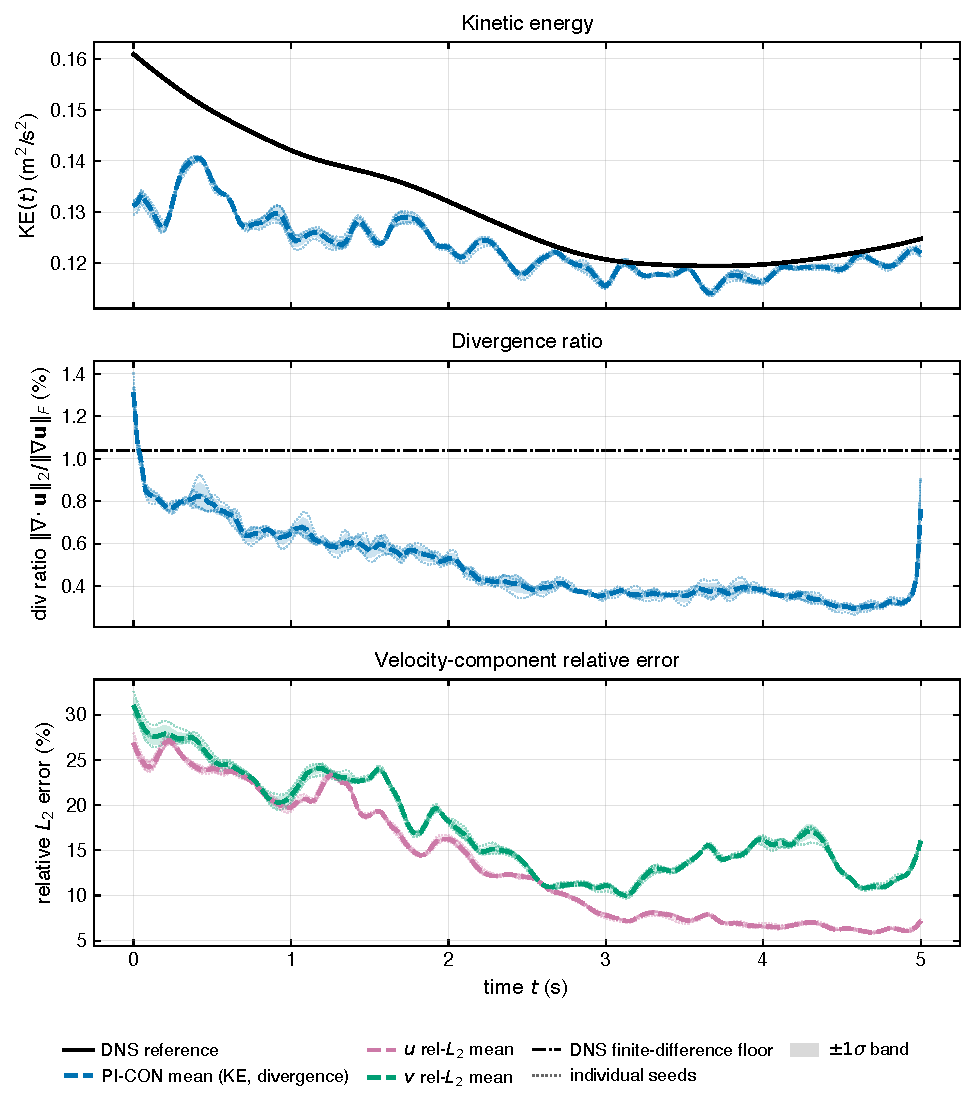
\includegraphics[width=\linewidth]{figures/results/main_trajectories.pdf}
    \caption{LES-pivot main-pipeline trajectory diagnostics over $n=5$ seeds (42, 1, 2, 3, 4), versus time $t$ (s). First panel: kinetic energy $\mathrm{KE}(t)$ (m$^2$/s$^2$). Second panel: divergence ratio $\Vert\nabla\!\cdot\!\mathbf{u}_{\rm pred}\Vert_2 / \Vert\nabla\mathbf{u}\Vert_F^{\rm DNS}$ (\%), with the DNS finite-difference floor. Third panel: $u$ and $v$ root-mean-square error (m/s). Fourth panel: DNS component magnitudes $\Vert u_{\rm DNS}\Vert_{\rm rms}$ and $\Vert v_{\rm DNS}\Vert_{\rm rms}$ (m/s), which are the denominators of the component relative $L_2$ errors reported in Table~\ref{tab:main_metrics}. In the first three panels the dashed line is the across-seed mean, dotted lines are individual seeds, and the shaded band is $\pm 1\sigma$; the DNS reference is solid.}
    \label{fig:main_trajectories}
\end{figure}

\begin{table}[!htbp]
    \centering
    \caption{Time-segment decomposition of the LES-pivot main result. Early: $t<1$~s; Mid: $1\le t<3$~s; Late: $t\ge 3$~s.}
    \label{tab:time_local}
    \small
    \begin{tabular}{lccc}
    \toprule
    \textbf{Metric} & \textbf{Early ($t<1$)} & \textbf{Mid ($1\le t<3$)} & \textbf{Late ($t\ge 3$)} \\
    \midrule
    $u$ rmse & 0.112 & 0.053 & 0.042 \\
    $v$ rmse & 0.102 & 0.051 & 0.033 \\
    $\omega$ rmse & 6.63 & 3.55 & 2.34 \\
    KE MAPE & $\sim 14\%$ & $\sim 5\%$ & $\sim 5\%$ \\
    \bottomrule
    \end{tabular}
\end{table}

\paragraph{Multi-seed statistical confirmation.}
\label{sec:statistical_significance}
The main result is checked against seed variability with an $n=5$ ensemble, which also provides a training-variability estimate.

\paragraph{Multi-seed training variability.}
The multi-seed training protocol follows a \emph{deep ensemble}~\cite{Lakshminarayanan2017DeepEnsembles}: training $n=5$ models from different random initialisations yields both a point estimate (the across-seed mean) and an empirical measure of training-induced variability (the across-seed standard deviation), capturing sensitivity to random initialisation and to the stochastic physics-collocation sampling schedule~\cite{Psaros2023UQ}. Here $n=5$ seeds yield a KE standard deviation of $0.11$ percentage points ($1.9\%$ relative scatter). This quantifies seed-and-collocation variability rather than a calibrated predictive uncertainty: no coverage or calibration of the spread is claimed.

To confirm the main result is not a seed artefact, the B3 LES-pivot configuration is trained over five seeds ($42, 1, 2, 3, 4$) at the main-pipeline $20\,000$-iteration budget. Table~\ref{tab:multiseed} reports per-seed values.

\begin{table}[!htbp]
    \centering
    \caption{Per-seed metrics for the B3 LES-pivot pipeline at $Re=10\,000$, $K=100$, $1024$ collocation points, $20\,000$ iterations. Last row: across-seed mean $\pm$ standard deviation. The KE, $u$, $v$, and $\omega$ errors are time-averaged over $t\in[0,T]$ (KE is MAPE); the $k_f$ amplitude ratio is reported at the final time $t=5$.}
    \label{tab:multiseed}
    \footnotesize
    \setlength{\tabcolsep}{3pt}
    \begin{tabularx}{\textwidth}{
        >{\raggedright\arraybackslash}p{1.6cm}
        >{\centering\arraybackslash}X
        >{\centering\arraybackslash}X
        >{\centering\arraybackslash}X
        >{\centering\arraybackslash}X
        >{\centering\arraybackslash}X
        >{\centering\arraybackslash}X
    }
    \toprule
    \textbf{Seed} & \textbf{KE \%} & \textbf{$u$ $L_2$ \%} & \textbf{$v$ $L_2$ \%} & \textbf{$\omega$ $L_2$ \%} & \textbf{div ratio \%} & \textbf{$k_f$ amp} \\
    \midrule
    $42$ ($_a$) & $5.9035$ & $13.59$ & $17.53$ & $41.66$ & $0.39$ & $0.9973$ \\
    $1$  ($_b$) & $5.6751$ & $13.74$ & $17.70$ & $41.95$ & $0.40$ & $0.9852$ \\
    $2$  ($_c$) & $5.6491$ & $13.63$ & $17.48$ & $41.67$ & $0.40$ & $0.9871$ \\
    $3$  ($_d$) & $5.7144$ & $13.66$ & $17.46$ & $41.83$ & $0.39$ & $0.9915$ \\
    $4$  ($_e$) & $5.5882$ & $13.65$ & $17.44$ & $41.75$ & $0.39$ & $0.9957$ \\
    \midrule
    \textbf{mean$\pm$std} & $\mathbf{5.71 {\pm} 0.11}$ & $\mathbf{13.65 {\pm} 0.06}$ & $\mathbf{17.52 {\pm} 0.10}$ & $\mathbf{41.79 {\pm} 0.12}$ & $\mathbf{0.39 {\pm} 0.006}$ & $\mathbf{0.991 {\pm} 0.005}$ \\
    \bottomrule
    \end{tabularx}
\end{table}

\paragraph{Reproducibility.}
The seed-to-seed KE standard deviation is $0.11$ percentage points ($1.9\%$ relative to the mean); all five seeds fall within a $0.32$ percentage-point window ($5.59$--$5.90\%$). Pointwise $u$-$L_2$ and $v$-$L_2$ are tighter still ($\sigma=0.06\%$ and $0.10\%$, both below $1\%$ relative scatter). The divergence ratio is reproducible to two decimal places ($0.39 \pm 0.006\%$), confirming it is a property of the architecture--AL recipe rather than any individual seed (\S\ref{sec:sub_dns_div}).

\paragraph{Architectural significance.}
The architectural advantage holds at budget parity. With all four ablation cells trained at the matched $1\,024$-collocation $20\,000$-iteration $n=5$-seed regime, a Welch $t$-test between B0 (Vanilla DeepONet, $8.23 \pm 0.22\%$) and B3 (Full PI-CON, $5.71 \pm 0.11\%$) gives a KE gap of $-2.52$ percentage points ($t=22.9$, $p=3.0\times10^{-7}$, Cohen's $d=14.5$): the gain is significant and not an artefact of seed count or iteration budget. The full $2\times2$ component decomposition appears with the ablation matrix (\S\ref{sec:baseline_comparison}).

\section{Field, Vorticity, and Low-Order Statistics}
\label{sec:visual}

\begin{figure}[!htbp]
    \centering
    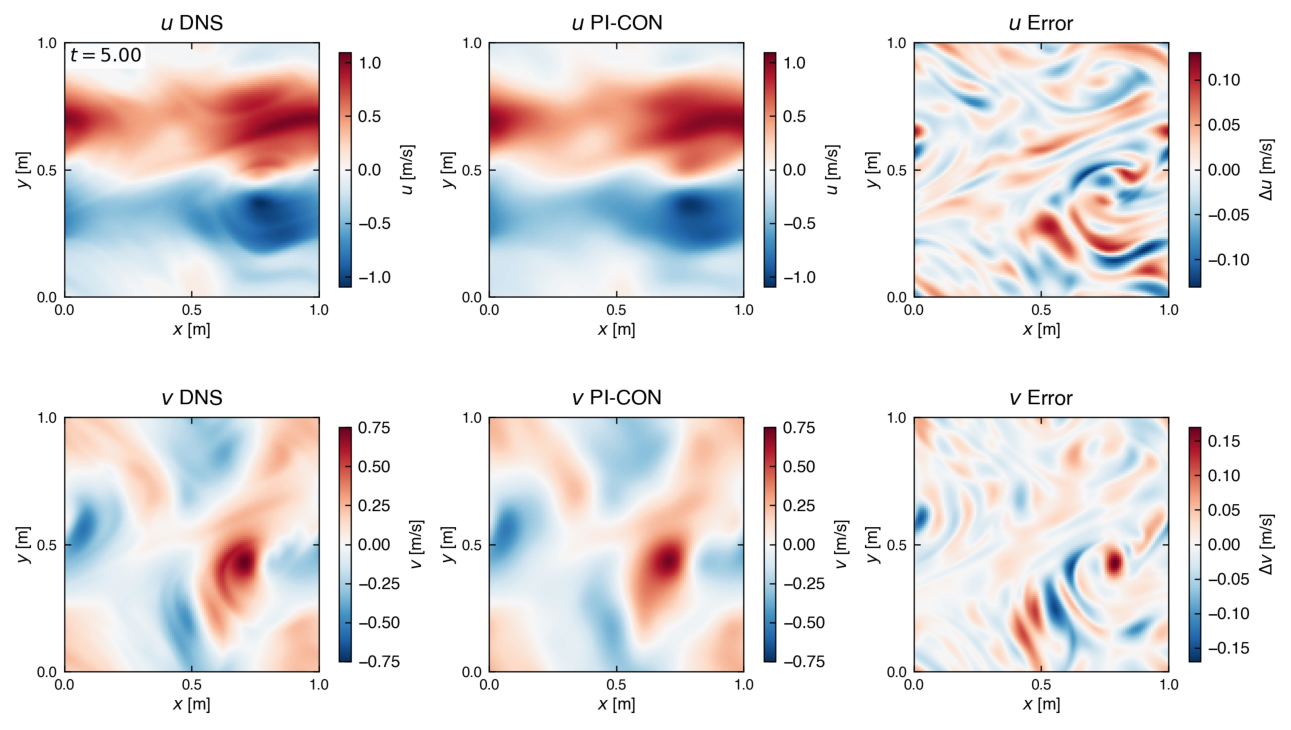
\includegraphics[width=0.95\linewidth]{figures/results/field_comparison_t5.pdf}
    \caption{Velocity and vorticity fields at $t=5$ (seed 42). Columns: DNS reference, PI-CON prediction, absolute error. Rows: $u$ (m/s), $v$ (m/s), vorticity $\omega$ (1/s).}
    \label{fig:field_t5}
\end{figure}

\begin{figure}[!htbp]
    \centering
    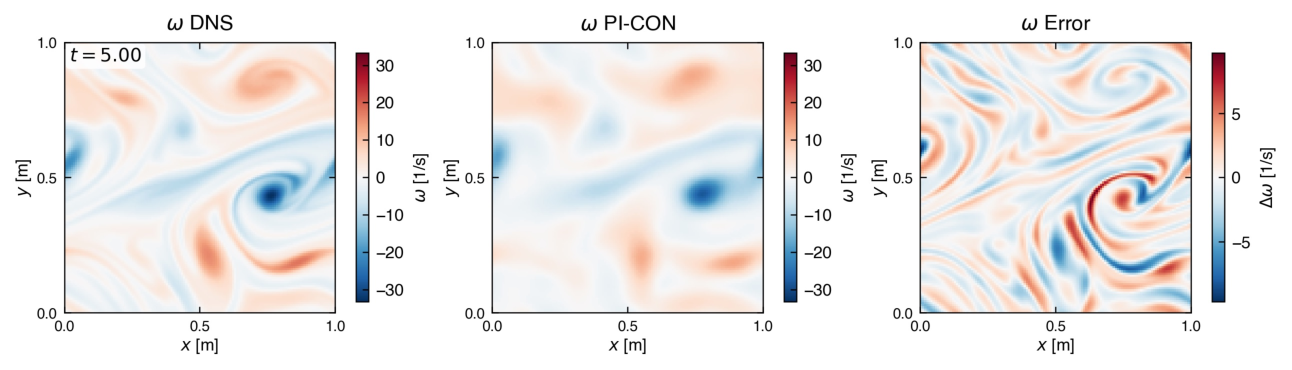
\includegraphics[width=0.92\linewidth]{figures/results/vorticity_comparison_t5.pdf}
    \caption{Vorticity fields at $t=5$ (seed 42). Left: DNS; middle: PI-CON prediction; right: error $\omega_{\rm pred} - \omega_{\rm DNS}$ (1/s). Axes: $x, y$ on $\Omega=[0,1]^2$ m$^2$. Left and middle share a colourbar; the error panel uses an independent symmetric scale.}
    \label{fig:vorticity_t5}
\end{figure}

Figure~\ref{fig:field_t5} compares $u$, $v$, and $\omega$ at $t=5$. PI-CON recovers the dominant DNS structures (large-scale shear bands in $u$ and energy-containing vortices in $v$) with the correct positions, signs, and amplitudes; residuals are fine-scale and structured rather than bulk offsets. The field is a low-pass reconstruction: energy-dominant large scales are recovered, while vorticity filaments and sharp cores are attenuated, matching the spectral roll-off in \S\ref{sec:spectrum}.

\paragraph{Discussion.}
The error structure in Figures~\ref{fig:field_t5}--\ref{fig:vorticity_t5} follows the $k^2$ amplification of $\omega$ relative to $u$ and $v$: vorticity is the hardest quantity to reconstruct under the $K=100$ budget and is reported as a diagnostic rather than a primary observable. The residual is spatially structured rather than random, pointing to a wavenumber-content limitation (\S\ref{sec:spectrum}). For engineering tasks driven by mean flow, kinetic energy, and dominant-structure positions, the $u$ and $v$ reconstruction in Figure~\ref{fig:field_t5} is adequate; tasks requiring fine-scale turbulence statistics (such as higher-order Reynolds-stress moments) need either more sensors or a different prior.

\paragraph{Low-order statistics.}
Beyond the instantaneous fields, the time- and span-averaged statistics quantify how well the reconstruction serves mean-flow monitoring. Figure~\ref{fig:mean_profile} reports the mean streamwise profile $\langle u\rangle_{x,t}(y)$ and the Reynolds shear stress $\langle u'v'\rangle_{x,t}(y)$, averaged over $x$ and the post-spin-up window $t\in[1,5]$~s. The mean profile agrees with DNS to $1.55\%$ relative $L_2$ error and the Reynolds shear stress to $8.61\%$; the two-lobe shear structure set by the $k_f=2$ forcing is reproduced in both amplitude and position. Low-order statistics fall well within the engineering target, supporting mean-flow and momentum-flux monitoring at the $K=100$ budget.

\begin{figure}[!htbp]
    \centering
    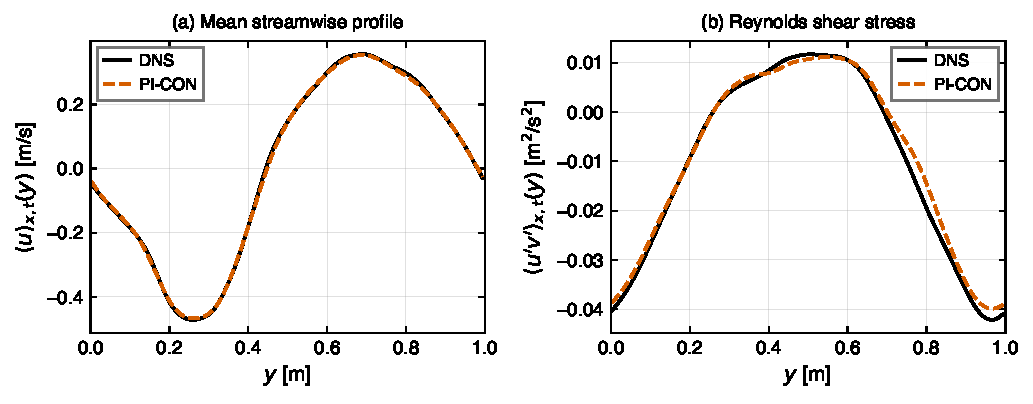
\includegraphics[width=\linewidth]{figures/results/mean_profile_reynolds.pdf}
    \caption{Low-order velocity statistics at $Re=10\,000$, $K=100$ (seed 42, LES-derived placement), averaged over $x$ and the window $t\in[1,5]$~s. (a) Mean streamwise profile $\langle u\rangle_{x,t}(y)$ (m/s) versus $y$ (m). (b) Reynolds shear stress $\langle u'v'\rangle_{x,t}(y)$ (m$^2$/s$^2$) versus $y$ (m). Solid: DNS; dashed: PI-CON.}
    \label{fig:mean_profile}
\end{figure}

\section{Spectral and Temporal Characterisation}
\label{sec:spectrum}

\paragraph{Energy spectrum evidence.}
\label{subsec:spectrum_evidence}

\begin{figure}[!htbp]
    \centering
    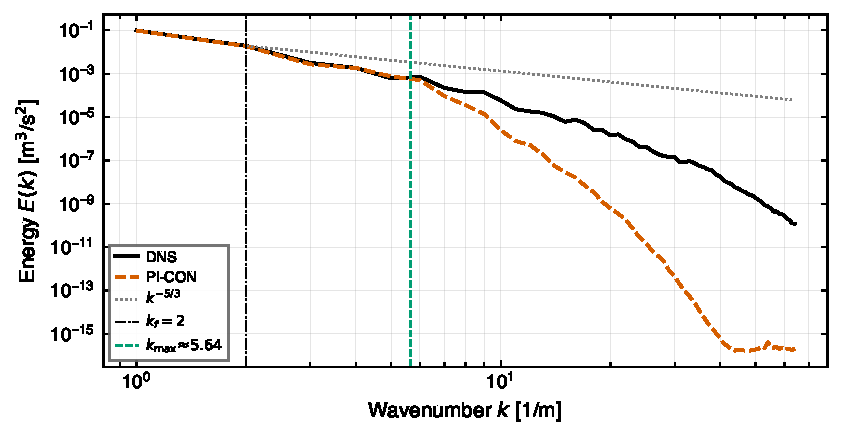
\includegraphics[width=0.92\linewidth]{figures/results/energy_spectrum.pdf}
    \caption{Radial energy spectrum at $t=5$ for the representative single seed (seed 42). Horizontal axis: wavenumber $k$ (1/m), log scale; vertical axis: radial energy spectrum $E(k)$ (m$^3$/s$^2$), log scale. DNS (solid black) and PI-CON prediction (dashed blue). Vertical dash-dotted line marks the forcing wavenumber $k_f = 2$; vertical dashed green line marks the sensor-count Nyquist scale $k_{\max}^{\rm sensor}\approx 5.64$.}
    \label{fig:spectrum}
\end{figure}

Figure~\ref{fig:spectrum} shows the radial energy spectrum at $t=5$. PI-CON matches the DNS spectrum within the sensor Nyquist band $k\le k_{\max}^{\rm sensor}\approx 5.64$ (carrying $\approx 99\%$ of the total energy at $t=5$); for $k\ge 16$ the prediction drops to a near-constant floor of $\approx 10^{-7}$, whereas the DNS continues a Kolmogorov-like cascade up to $k\sim 64$.

Figure~\ref{fig:band_err} reports the per-band relative error against time as the $n=5$ seed mean. The low band ($k\le 5$) decays over the window to a median of $2.5\%$ (range $0.07$--$14.9\%$ for $t>0$) and reaches near-zero at several instants. For $t\ge 0.5$\,s the high band ($k>16$) holds a median of $99.9\%$ (range $99.1$--$100.0\%$), the level a band carries when the reconstruction places no energy in it, while the mid band ($5<k\le 16$) holds a median of $53.5\%$ (range $41.7$--$71.0\%$). (The $t=0$ frame is excluded because high-$k$ energy there is near-zero, making relative error singular.)

\paragraph{Discussion.}
The high-$k$ deviation is the expected signature of a sensor-limited reconstruction rather than a model defect. At $K=100$ the available measurements constrain the energy-dominant low-wavenumber band but do not independently determine the mid and high bands. The $K$-scaling experiment in \S\ref{subsec:nyquist_scaling} provides further evidence: the reconstruction bandwidth tracks the sensor-count Nyquist scale.

\begin{figure}[!htbp]
    \centering
    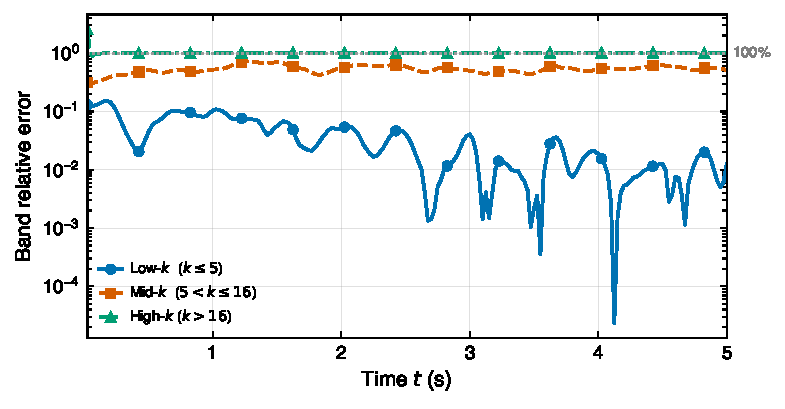
\includegraphics[width=0.85\linewidth]{figures/results/band_energy_rel_error_vs_time.pdf}
    \caption{Band-energy relative error (dimensionless) vs.\ time $t$ (s), LES-derived placement. Mean (solid, markers) $\pm 1\sigma$ (shaded) over $n=5$ seeds, with individual seeds dotted. Bands: low-$k$ ($k\le 5$, sensor-count Nyquist scale), mid-$k$ ($5<k\le 16$), high-$k$ ($k>16$). The $t=0$ frame is excluded.}
    \label{fig:band_err}
\end{figure}

\paragraph{Enstrophy and dissipation under the spectral cutoff.}
The band-limited reconstruction carries a direct consequence for vorticity-derived statistics. Figure~\ref{fig:dissipation_budget} compares the enstrophy $\mathcal{Z}(t)$ against DNS, with the dissipation rate $\varepsilon=2\nu\mathcal{Z}$ on the right axis as a constant rescaling. The reconstruction lies below the DNS reference by $26.0 \pm 0.2\%$ ($n=5$ seeds) on the post-spin-up window $t\ge 1$~s, because the mid/high-wavenumber content beyond the $K=100$ Nyquist scale carries enstrophy weighted by $k^2$. The deficit follows the spectral roll-off at $k\ge 16$ (Fig.~\ref{fig:spectrum}) and the $\omega$ relative error of Table~\ref{tab:main_metrics}: kinetic energy, concentrated at low wavenumbers, is recovered, while enstrophy-level statistics remain sensor-bounded.

\begin{figure}[!htbp]
    \centering
    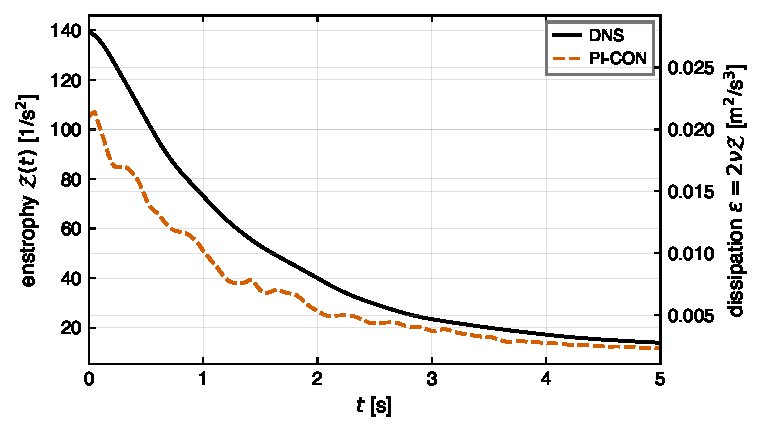
\includegraphics[width=\linewidth]{figures/results/dissipation_budget.pdf}
    \caption{Enstrophy $\mathcal{Z}(t)$ (left axis, 1/s$^2$) versus time $t$ (s), LES-derived placement; the right axis shows the dissipation rate $\varepsilon=2\nu\mathcal{Z}$ (m$^2$/s$^3$), a constant rescaling of the left axis. Solid: DNS reference (identical across seeds). Dashed: PI-CON mean over $n=5$ seeds, with the $\pm 1\sigma$ band shaded and individual seeds dotted.}
    \label{fig:dissipation_budget}
\end{figure}

\paragraph{Forcing-mode ($k = k_f = 2$) diagnostic.}
Because $k_f = 2$ lies inside the sensor-resolvable low band, the forcing-mode amplitude and phase check the energy-injection scale. Over $n=5$ seeds, after the initial-condition window ($t\ge 1$~s), the amplitude ratio holds near unity (mean $0.99$) and the phase error stays within $0.09$~rad ($\approx 5^\circ$), ending at $-0.013$~rad (Fig.~\ref{fig:kf_mode}), recovering the forced response; broadband pointwise fidelity is reported separately in Table~\ref{tab:main_metrics}.

\begin{figure}[!htbp]
    \centering
    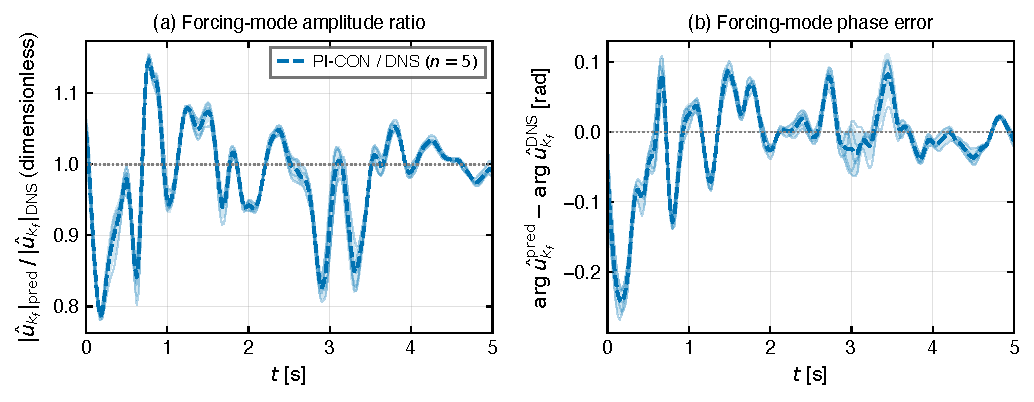
\includegraphics[width=\linewidth]{figures/results/kf_mode_diagnostic.pdf}
    \caption{Forcing-mode ($k_f = 2$) reconstruction over $n=5$ seeds, LES-derived placement. (a) Amplitude ratio $|\hat{u}_{k_f}|_{\rm pred}/|\hat{u}_{k_f}|_{\rm DNS}$ (dimensionless) versus time $t$ (s). (b) Phase error $\arg\hat{u}_{k_f}^{\rm pred}-\arg\hat{u}_{k_f}^{\rm DNS}$ (rad) versus $t$ (s). Dashed: across-seed mean; dotted: individual seeds; shaded: $\pm 1\sigma$; dotted grey lines mark the ideal amplitude ratio $1$ and zero phase error.}
    \label{fig:kf_mode}
\end{figure}

\paragraph{Temporal dynamics.}
Because the CfC branch encodes the sensor time series rather than reconstructing each frame independently, the reconstruction is also assessed in the time domain. Figure~\ref{fig:temporal_consistency} shows a velocity probe trace at the domain centre and the spatially-averaged temporal autocorrelation $R_{uu}(\tau)$. The probe trace follows the DNS instantaneous evolution, and the autocorrelation reproduces the DNS decorrelation: the $1/e$ time is $0.40$~s for PI-CON against $0.375$~s for DNS. The reconstruction recovers the temporal decorrelation structure, not only per-frame spatial statistics. A forward LES initialised from the same field departs from the DNS over this window (Fig.~\ref{fig:temporal_consistency}a, dotted), so the instantaneous probe evolution is recovered from the sparse sensor stream, not from a forward simulation.

\begin{figure}[!htbp]
    \centering
    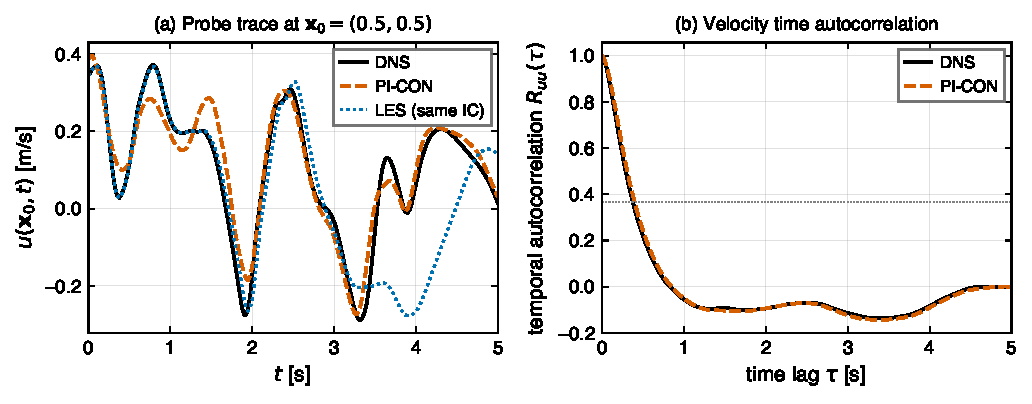
\includegraphics[width=\linewidth]{figures/results/temporal_consistency.pdf}
    \caption{Temporal behaviour at $Re=10\,000$, $K=100$ (seed 42, LES-derived placement). (a) Velocity probe trace $u(\mathbf{x}_0,t)$ (m/s) at the domain centre $\mathbf{x}_0=(0.5,0.5)$ versus $t$ (s); solid: DNS, dashed: PI-CON, dotted: a forward LES from the same initial field. (b) Spatially-averaged temporal autocorrelation $R_{uu}(\tau)$ (dimensionless) versus time lag $\tau$ (s) for DNS (solid) and PI-CON (dashed); the horizontal dotted line marks the $1/e$ level.}
    \label{fig:temporal_consistency}
\end{figure}

\section{Architectural Ablation}
\label{sec:supporting_comparisons}

This section attributes the main result to its components: a divergence diagnostic confirming the continuity constraint is active, then the $2\times2$ architecture ablation under the final PI-CON training protocol.

\paragraph{Divergence diagnostic.}
\label{sec:sub_dns_div}
The main pipeline applies Augmented-Lagrangian (AL) continuity at $\rho=0.1$, and the reconstructed field attains divergence ratio $0.39 \pm 0.006\%$ over $n=5$ seeds (Table~\ref{tab:main_metrics}): a physical-convergence check that the constraint is active, carrying no comparative meaning against DNS. The finite-difference operator is bandwidth-dependent: it registers $1.04\%$ on the full-cascade DNS field but $0.38\%$ once that field is band-limited to $k\le 16$ (\S\ref{subsec:dns_verification}); at matched bandwidth the reconstruction's $0.39\%$ sits at the $k\le 16$ DNS level, so the constraint drives divergence to the finite-difference floor permitted by its resolved scales rather than below DNS. The same recipe attains $0.37\%$ at $Re=10^{6}$, consistent across Reynolds numbers. The AL-strength sweep selecting $\rho=0.1$ is a hyperparameter diagnostic reported in Appendix~\ref{app:diagnostic_ablation_forward_cfd}.

\paragraph{Architectural ablation matrix.}
\label{sec:baseline_comparison}
The ablation isolates the contribution of CfC and cross-attention under the final common supervision regime. A $2\times2$ matrix toggles CfC and cross-attention independently: Vanilla DeepONet (B0), CfC-only (B1), Cross-attention-only (B2), and Full PI-CON (B3). The four cells share the supervision regime of \S\ref{sec:engineering_constraint}, the optimizer, the LES $T=50$ sensor placement, and $1024$ physics-collocation points used by the main pipeline (\S\ref{sec:main_result}). Engineering-transferable interpolation baselines (RBF, IDW, divergence-free trigonometric least squares) are compared against PI-CON in Appendix~\ref{app:fair_baselines}: PI-CON reduces pointwise $u$ rel-$L_2$ by $47$--$74\%$ relative to them despite their lower KE, which comes from over-smoothing toward the inter-sensor mean rather than better reconstruction.

\begin{table}[!htbp]
    \centering
    \caption{$2\times2$ architectural ablation at $Re=10\,000$, $K=100$, LES $T=50$ placement, $1024$ collocation points. All rows report mean $\pm$ standard deviation over $n=5$ seeds $\{42,1,2,3,4\}$ at $20\,000$ iterations. Relative-error metrics are percentages.}
    \label{tab:ablation_22matrix}
    \footnotesize
    \setlength{\tabcolsep}{3pt}
    \begin{tabularx}{\textwidth}{
        >{\raggedright\arraybackslash}p{4.0cm}
        >{\centering\arraybackslash}X
        >{\centering\arraybackslash}X
        >{\centering\arraybackslash}X
        >{\centering\arraybackslash}X
        >{\centering\arraybackslash}p{1.3cm}
    }
    \toprule
    \textbf{Variant} & \textbf{$u$ $L_2$ \%} & \textbf{$v$ $L_2$ \%} & \textbf{$\omega$ $L_2$ \%} & \textbf{KE \%} & \textbf{Params} \\
    \midrule
    B0 Vanilla DeepONet     & $15.42 {\pm} 0.11$ & $20.28 {\pm} 0.12$ & $45.44 {\pm} 0.26$ & $8.23 {\pm} 0.22$ & $1.28$\,M \\
    B1 CfC only             & $18.05 {\pm} 0.14$ & $24.26 {\pm} 0.30$ & $51.14 {\pm} 0.31$ & $9.23 {\pm} 0.51$ & $3.14$\,M \\
    B2 Cross-attention only & $14.64 {\pm} 0.12$ & $19.39 {\pm} 0.09$ & $44.32 {\pm} 0.17$ & $7.03 {\pm} 0.14$ & $2.74$\,M \\
    B3 Full PI-CON (Ours)   & $\mathbf{13.65 {\pm} 0.06}$ & $\mathbf{17.52 {\pm} 0.10}$ & $\mathbf{41.79 {\pm} 0.12}$ & $\mathbf{5.71 {\pm} 0.11}$ & $3.14$\,M \\
    \bottomrule
    \end{tabularx}
\end{table}

\paragraph{Architectural ranking under the main pipeline.}
With all four cells trained at the matched $20\,000$-iteration, $n=5$-seed budget, the KE ordering is B3 ($5.71 \pm 0.11\%$) $\prec$ B2 ($7.03 \pm 0.14\%$) $\prec$ B0 ($8.23 \pm 0.22\%$) $\prec$ B1 ($9.23 \pm 0.51\%$). Seed-paired Welch $t$-tests confirm every gap to B3 is significant: $-2.52$ percentage points versus B0 ($t=22.9$, $p=3.0\times10^{-7}$), $-3.52$ versus B1 ($t=15.1$, $p=5.5\times10^{-5}$), and $-1.32$ versus B2 ($t=16.3$, $p=2.4\times10^{-7}$). Decomposing the $2\times2$ on the absolute KE scale about the B0 reference cell (where the decomposition is additive) separates a cross-attention main effect of $-1.20$ percentage points, a CfC main effect of $+1.00$, and a CfC$\times$cross-attention interaction of $-2.32$, summing to the $-2.52$ B3$-$B0 total. Cross-attention is the dominant lever. CfC raises KE error on its own (mean-pool aggregation in B1 erodes the per-query specificity that physics-residual sampling supplies) but carries a large negative interaction, so it lowers error only in combination with the cross-attention readout.

\section{Sensing-Configuration Study}
\label{sec:sensing_study}

Three sensing-configuration levers govern reconstruction quality: sensor count, placement, and measurement noise. This section quantifies the sensor count and its Nyquist scale, then reports placement and noise robustness.

\subsection{Nyquist-Aligned K-Scaling}
\label{subsec:nyquist_scaling}

The most direct test of the information-limited interpretation varies sensor count while keeping the LES-derived placement principle fixed. For point sensors on a two-dimensional domain, the sensor-count Nyquist estimate gives
\begin{equation}
    k_{\max}^{\rm sensor} \;\approx\; \sqrt{K/\pi},
\end{equation}
a scale for the reconstructable band rather than a hard cutoff. It counts each sensor as a single sample, whereas the two measured velocity components $(u,v)$ at the divergence-free-constrained locations push the strict linear-observability limit somewhat higher (for $K=100$ the sensing matrix stays full-rank up to $k\lesssim 8$, Appendix~\ref{app:info_ceiling_diagnostics}). Raising $K$ from $100$ to $200$ and $400$ moves this scale from $\approx 5.64$ to $7.98$ and $11.28$.

Read against the DNS energy distribution, the scale locates how much energy lies within reach of each sensor count. Figure~\ref{fig:nyquist_recoverability} integrates the DNS energy CDF at $t=5$ over the $|\mathbf{k}|\le k_{\max}^{\rm sensor}$ disk, giving $98.9\%$, $99.7\%$, and $99.9\%$ of total kinetic energy at $K=100$, $200$, and $400$. These fractions report the energy available below the sensor-count scale, not a proof that higher-$k$ energy is unrecoverable. The information-limited reading rests instead on the empirical cutoff tracking $\sqrt{K/\pi}$ as $K$ grows.

\begin{figure}[!htbp]
    \centering
    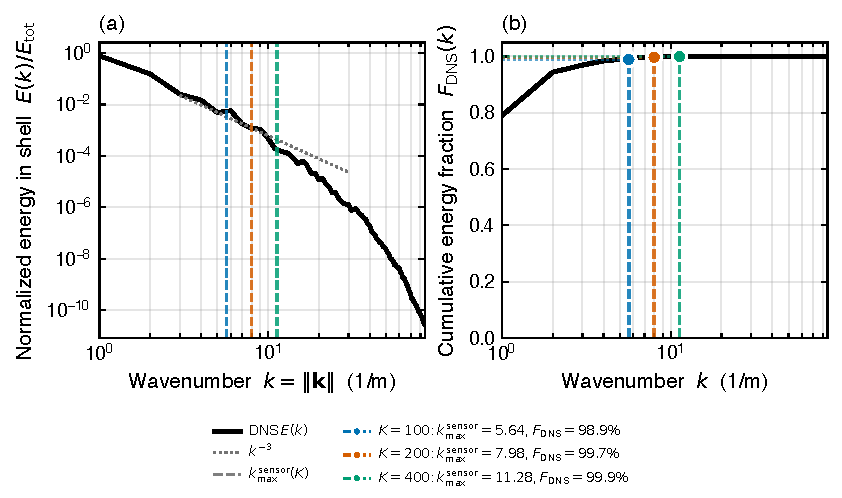
\includegraphics[width=0.95\linewidth]{figures/results/nyquist_recoverability.pdf}
    \caption{DNS energy available within the sensor-count Nyquist scale $\sqrt{K/\pi}$ for $K$ point velocity sensors ($Re=10^4$, $N=256$, $t=5$~s). (a)~Radial DNS energy spectrum $E(k)/E_{\rm tot}$ (dimensionless) versus wavenumber $k$ (1/m), with the $k^{-3}$ enstrophy-cascade reference (dotted; the forward-cascade slope for $k>k_f$) and Nyquist scales $k_{\max}^{\rm sensor}=\sqrt{K/\pi}$ (vertical dashed, colour-coded by $K$). (b)~Cumulative DNS energy fraction $F_{\rm DNS}(k)$ (dimensionless) versus $k$ (1/m); markers locate $F_{\rm DNS}(k_{\max}^{\rm sensor})$ for $K\in\{100,200,400\}$.}
    \label{fig:nyquist_recoverability}
\end{figure}

Table~\ref{tab:k_scaling_nyquist} reports the empirical reconstruction following this Nyquist-predicted bandwidth expansion.

\begin{table}[!htbp]
    \centering
    \caption{Sensor-count scaling against the Nyquist scale $\sqrt{K/\pi}$. LES-derived QR-pivot sensors, seed 42, $20\,000$ iterations; metrics at $t=5$. The $K=400$ run uses $512$ collocation points (memory budget).}
    \label{tab:k_scaling_nyquist}
    \small
    \setlength{\tabcolsep}{5pt}
    \begin{tabular}{lccc}
    \toprule
    \textbf{Quantity} & \textbf{$K=100$} & \textbf{$K=200$} & \textbf{$K=400$} \\
    \midrule
    Nyquist $k_{\max}^{\rm sensor}$ & 5.64 & 7.98 & 11.28 \\
    KE MAPE & 5.90\% & 2.47\% & \textbf{1.76\%} \\
    $u$ rel-$L_2$ & 7.10\% & 4.95\% & 4.11\% \\
    $v$ rel-$L_2$ & 16.08\% & 10.30\% & 8.64\% \\
    $\omega$ rel-$L_2$ & 38.03\% & 31.36\% & 29.29\% \\
    $k_f$ amplitude ratio & 0.969 & \textbf{0.998} & 0.975 \\
    \bottomrule
    \end{tabular}
\end{table}

\begin{figure}[!htbp]
    \centering
    \begin{subfigure}[t]{0.32\linewidth}
        \centering
        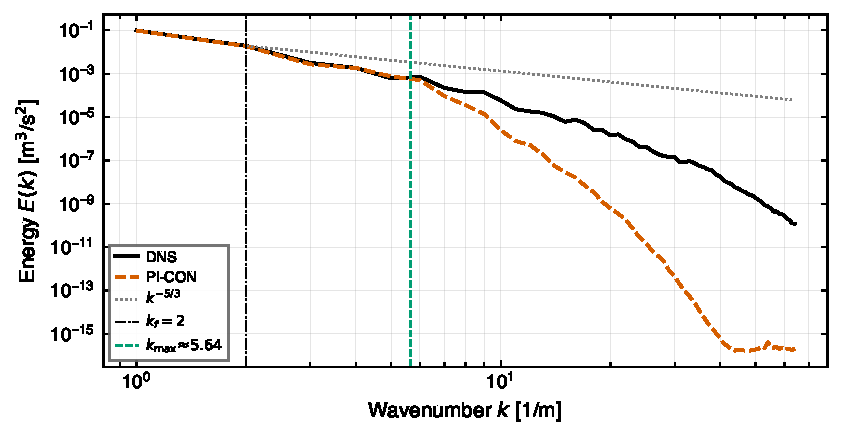
\includegraphics[width=\linewidth]{figures/results/spectrum_K100_nyquist.pdf}
        \caption{$K=100$, $k_{\max}^{\rm sensor}\approx 5.64$}
        \label{fig:spectrum_K100}
    \end{subfigure}\hfill
    \begin{subfigure}[t]{0.32\linewidth}
        \centering
        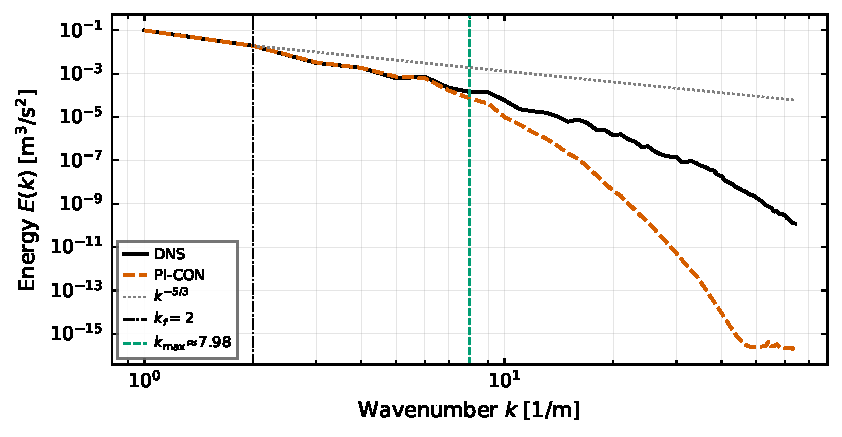
\includegraphics[width=\linewidth]{figures/results/spectrum_K200_nyquist.pdf}
        \caption{$K=200$, $k_{\max}^{\rm sensor}\approx 7.98$}
        \label{fig:spectrum_K200}
    \end{subfigure}\hfill
    \begin{subfigure}[t]{0.32\linewidth}
        \centering
        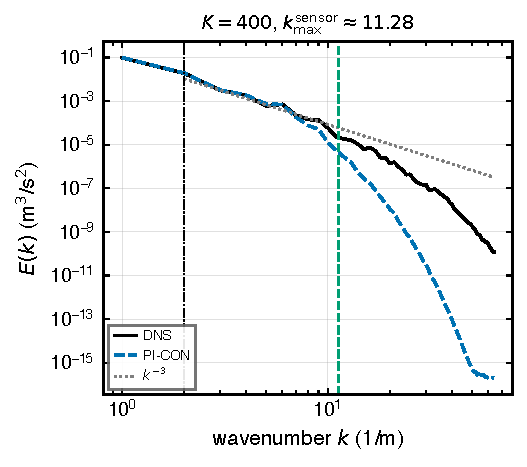
\includegraphics[width=\linewidth]{figures/results/spectrum_K400_nyquist.pdf}
        \caption{$K=400$, $k_{\max}^{\rm sensor}\approx 11.28$}
        \label{fig:spectrum_K400}
    \end{subfigure}
    \caption{Radial energy spectrum $E(k)$ (m$^3$/s$^2$) versus wavenumber $k$ (1/m) at $t=5$ for three sensor budgets. Each panel: DNS (solid black), PI-CON (dashed blue), $k^{-3}$ enstrophy-cascade reference (dotted grey; the forward-cascade slope for $k>k_f$), forcing $k_f = 2$ (dash-dotted black), sensor Nyquist $k_{\max}^{\rm sensor}=\sqrt{K/\pi}$ (dashed green). LES-derived QR-pivot, seed $42$, $20\,000$ iterations.}
    \label{fig:k_scaling_spectra}
\end{figure}

The agreement is qualitative but clear: at $K=100$ the $\sqrt{K/\pi}$ scale sits near the low/mid-band boundary, $K=200$ pushes it close to $k\approx 8$, and $K=400$ reaches into the inertial-range content (Figure~\ref{fig:k_scaling_spectra}). KE error drops by $70\%$ between $K=100$ and $K=400$ ($5.90\%\to1.76\%$; the $K=100$ value is the seed-42 single run, whose $n=5$ mean is $5.71\%$, Table~\ref{tab:multiseed}). The observed KE ratios relative to $K=100$ are $0.42$ at $K=200$ and $0.30$ at $K=400$. The Nyquist relation $k_{\max}^{\rm sensor}\propto\sqrt{K}$, under which the unresolved energy above the cutoff scales as $k_{\max}^{-2}\propto 1/K$, predicts ratios of $100/K = 0.50$ and $0.25$ respectively, placing the measured curve within $20\%$ of this scaling estimate. Because the $K=400$ run uses fewer collocation points, the three-point curve should not be read as a strict fit; it shows that higher fidelity comes from sensor bandwidth expansion, not from architecture search.


\subsection{Information-Ceiling Summary}
\label{sec:info_limit_summary}

The $K=100$ result should be read against the sensor information ceiling rather than as an unconstrained full-field regression problem. A wavelet sparsity diagnostic, a sensing-matrix rank calculation, and a spectral-truncation bound point to the same interpretation: the low-wavenumber band is observable enough to support engineering KE and mean-flow monitoring, while mid- and high-wavenumber content remains underdetermined at this sensor budget. The B3 multi-seed KE error ($5.71\%$) maps to an effective spectral cutoff $k_{\rm cut}\approx 4.7$ and the $k^2$-weighted vorticity error to $k_{\rm cut}\approx 7.8$ (Appendix~\ref{app:info_ceiling_diagnostics}); the two bracket the sensor Nyquist estimate $k_{\max}^{\rm sensor}\approx 5.64$, as the sensor-count criterion of \S\ref{sec:research_questions} requires. Closing the remaining mid/high-band error therefore requires more sensors or extra modalities, not another architecture-side loss term.

The detailed wavelet, SVD, and spectral-truncation diagnostics are collected in Appendix~\ref{app:info_ceiling_diagnostics}.

\subsection{Sensor Placement Analysis}
\label{sec:placement_analysis}

Placement strategy contributes a variance source larger than training stochasticity at fixed $K=100$. Table~\ref{tab:placement_strategy_new} summarises the final-protocol placement comparison: DNS-oracle and LES-derived placements differ only in sensor-placement source and are both trained over $n=5$ random seeds at $20\,000$ iterations (Table~\ref{tab:main_metrics}); random placement is repeated over $n=5$ placement seeds with training seed fixed to isolate placement variance.

\begin{table}[!htbp]
    \centering
    \caption{Final-protocol placement comparison at $Re=10\,000$, $K=100$, B3, $1024$ collocation points, $20\,000$ iterations. DNS-oracle and LES-derived placements report training-seed mean $\pm$ standard deviation. Random placement reports placement-seed mean $\pm$ standard deviation with training seed fixed at $42$. In all rows the sensor \emph{values} are read from the DNS field that stands in for the real-world flow (at the $K$ sensor positions only); the second column marks only whether \emph{placement} additionally requires the DNS \emph{full field}.}
    \label{tab:placement_strategy_new}
    \footnotesize
    \setlength{\tabcolsep}{3pt}
    \begin{tabularx}{\textwidth}{
        >{\raggedright\arraybackslash}p{3.4cm}
        >{\centering\arraybackslash}X
        >{\centering\arraybackslash}X
        >{\centering\arraybackslash}X
        >{\centering\arraybackslash}X
    }
    \toprule
    \textbf{Placement strategy} & \textbf{DNS \emph{full field} for placement?} & \textbf{KE \%} & \textbf{$u$ $L_2$ \%} & \textbf{Interpretation} \\
    \midrule
    DNS QR-pivot oracle & Yes & $\mathbf{4.68 \pm 0.06}$ & $15.34 \pm 0.06$ & non-deployable lower-KE reference \\
    LES-derived QR-pivot & No & $5.71 \pm 0.11$ & $\mathbf{13.65 \pm 0.06}$ & main deployable placement \\
    Random uniform & No & $7.95 \pm 0.68$ & $17.20 \pm 1.42$ & no-placement-effort reference \\
    \bottomrule
    \end{tabularx}
\end{table}

\paragraph{Strategy comparison.}
All three strategies stay below the $10\%$ KE engineering target. The DNS oracle gives the lowest integral KE error ($4.68\%$), but the LES-derived placement gives lower pointwise velocity error ($u$ rel-$L_2$ $13.65\%$ vs.\ $15.34\%$) while needing no DNS full field to place the sensors. Random placement remains feasible ($7.95\%$ KE) but less reliable: placement changes reliability more than feasibility. The final pipeline adopts LES-derived QR-pivot placement as the deployable reference: it approaches the DNS oracle without needing a DNS full field for placement, and improves over random placement by $2.24$ KE percentage points.

\label{sec:placement_variance}

To estimate placement-induced variance separately from training stochasticity, the random-uniform strategy is repeated at $n=5$ placement seeds ($42, 1, 2, 3, 4$) with the training seed held at $42$.

\begin{table}[!htbp]
    \centering
    \caption{Random $K=100$ placement variance at $Re=10\,000$, B3, $1024$ collocation points, $20\,000$ iterations, training seed $42$. Each placement seed selects $K=100$ uniformly-random positions on the $256^2$ grid. Error columns: relative-error percentages (KE is MAPE); divergence ratio $= \Vert\nabla\!\cdot\!\mathbf{u}\Vert_2 / \Vert\nabla\mathbf{u}\Vert_F^{\rm DNS}$.}
    \label{tab:placement_variance}
    \footnotesize
    \setlength{\tabcolsep}{3pt}
    \begin{tabularx}{\textwidth}{
        >{\raggedright\arraybackslash}p{1.8cm}
        >{\centering\arraybackslash}X
        >{\centering\arraybackslash}X
        >{\centering\arraybackslash}X
        >{\centering\arraybackslash}X
        >{\centering\arraybackslash}X
    }
    \toprule
    \textbf{Placement seed} & \textbf{KE \%} & \textbf{$u$ $L_2$ \%} & \textbf{$v$ $L_2$ \%} & \textbf{div ratio \%} & \textbf{$k_f$ amp} \\
    \midrule
    $42$ & $7.24$            & $16.14$ & $20.33$ & $0.37$ & $\mathbf{1.001}$ \\
    $1$  & $\mathbf{9.18}$\,$^\dagger$ & $19.80$ & $25.64$ & $0.34$ & $0.941$ \\
    $2$  & $7.89$            & $16.48$ & $20.86$ & $0.36$ & $0.962$ \\
    $3$  & $8.03$            & $16.10$ & $20.16$ & $0.35$ & $0.966$ \\
    $4$  & $7.40$            & $17.47$ & $21.11$ & $0.34$ & $0.995$ \\
    \midrule
    \textbf{mean$\pm$std} & $\mathbf{7.95 {\pm} 0.68}$ & $17.20 {\pm} 1.42$ & $21.62 {\pm} 2.07$ & $\mathbf{0.35 {\pm} 0.01}$ & $0.973 {\pm} 0.024$ \\
    \bottomrule
    \end{tabularx}
    \\[2pt]
    \footnotesize $^\dagger$Outlier; random placement occasionally hits a configuration with poor spatial coverage.
\end{table}

\paragraph{Placement versus training variance.}
The two five-seed estimates yield $\sigma_{\rm training}=0.11\%$ (LES $T=50$, Table~\ref{tab:multiseed}) and $\sigma_{\rm placement}=0.68\%$ (random uniform, Table~\ref{tab:placement_variance}); placement variance dominates training stochasticity by
\begin{equation}
    \sigma_{\rm placement}/\sigma_{\rm training} \;\approx\; 6.2\times.
    \label{eq:placement_dominance}
\end{equation}
The ratio in \eqref{eq:placement_dominance} shows that LES-derived placement improves both the mean (KE $5.71\%$ vs.\ $7.95\%$, $\Delta=2.24$ percentage points, Welch $z \approx 3.3$, $p<0.01$) and the reproducibility ($6.2\times$ tighter), so engineering deployment should prioritise placement optimisation over training repetition. Divergence ratio stays at $0.35 \pm 0.01\%$ across all five placement seeds: the divergence diagnostic (\S\ref{sec:sub_dns_div}) is placement-invariant within the random-uniform family.

\paragraph{Field alignment does not improve placement.}
The placement LES is an independent, long-horizon realisation (\S\ref{sec:les_placement}). Initialising LES from the DNS field might seem preferable because it tracks the DNS pointwise for about one eddy-turnover time (Fig.~\ref{fig:les_predictability}), but Table~\ref{tab:placement_dnsinit} shows the opposite. A DNS-initialised LES integrated only to $t=5$ gives worse placement (KE $9.12\%$) than the long-horizon random-IC $T=50$ LES ($5.90\%$) at the same training seed. QR-pivot placement depends on leading POD modes, so a short DNS-seeded spin-down trajectory is less useful than a longer attractor sample. The dns-init run also requires a DNS field to seed and is diagnostic only.

\begin{table}[!htbp]
    \centering
    \caption{Field-aligned versus long-horizon sensor placement at $Re=10\,000$, $K=100$, B3, $1024$ collocation points, $20\,000$ iterations, single training seed $42$. The $t=5$ dns-init LES is initialised from the DNS field, so it tracks the DNS pointwise at early time, but it is a diagnostic (it needs a DNS field to seed), not a deployable option. KE is MAPE (percent); $\tau$ denotes the eddy-turnover time.}
    \label{tab:placement_dnsinit}
    \small
    \begin{tabular}{llc}
    \toprule
    \textbf{Placement source} & \textbf{POD window} & \textbf{KE \%} \\
    \midrule
    LES $T=50$, random IC (deployable)         & $\sim 22\,\tau$  & $5.90$ \\
    LES $t=5$, dns-init (field-aligned; diag.) & $\sim 2.5\,\tau$ & $9.12$ \\
    \bottomrule
    \end{tabular}
\end{table}

\subsection{Sensor Noise Robustness}
\label{sec:noise_robustness}

Because the main pipeline relies on measured sensor time series rather than full-field supervision, moderate observation noise must not dominate reconstruction. Table~\ref{tab:noise_robustness} reports the response to per-channel Gaussian noise at $1$--$10\%$ of the sensor standard deviation, with the LES-derived layout and final $20\,000$-iteration, $1024$-collocation training setup fixed. The sweep uses $n=5$ seeds at each noise level and supports O3 by testing whether the trained recipe remains within the engineering target under controlled additive perturbations.

\begin{table}[!htbp]
    \centering
    \caption{Sensor-noise robustness of the LES-pivot pipeline under the final PI-CON protocol ($20\,000$ iterations, $1024$ collocation, $n=5$ seeds per noise level). Noise level is relative to the per-channel sensor standard deviation; $\Delta$~KE is measured against the clean final-protocol baseline.}
    \label{tab:noise_robustness}
    \small
    \setlength{\tabcolsep}{5pt}
    \begin{tabular}{lccccc}
    \toprule
    \textbf{Noise $\sigma$} & \textbf{KE \%} & \textbf{$\Delta$ KE} & \textbf{$u$ $L_2$ \%} & \textbf{$v$ $L_2$ \%} & \textbf{div ratio \%} \\
    \midrule
    Clean & $5.71 {\pm} 0.11$ & -- & $13.65 {\pm} 0.06$ & $17.52 {\pm} 0.10$ & $0.39 {\pm} 0.006$ \\
    1\%  & $5.75 {\pm} 0.08$ & $+0.04$ & $13.66$ & $17.57$ & $0.40$ \\
    3\%  & $5.81 {\pm} 0.03$ & $+0.10$ & $13.74$ & $17.70$ & $0.40$ \\
    5\%  & $5.92 {\pm} 0.08$ & $+0.21$ & $13.90$ & $17.92$ & $0.42$ \\
    10\% & $6.08 {\pm} 0.21$ & $+0.37$ & $14.49$ & $18.77$ & $0.46$ \\
    \bottomrule
    \end{tabular}
\end{table}

The aggregate trend is monotone: increasing sensor noise raises KE error, pointwise error, vorticity error, and divergence ratio. Even at $10\%$ sensor noise, however, the KE error remains $6.08 \pm 0.21\%$, well below the $10\%$ engineering threshold. This supports the deployment criterion without relying on the older single-seed regularisation artefact.

\section{Higher-Reynolds Feasibility}
\label{sec:cross_reynolds}

The same architecture, with the sensor budget and model capacity retuned, is applied at $Re=10^{6}$ to probe whether the approach remains feasible two orders of magnitude higher in Reynolds number.

At higher Reynolds numbers the spatial under-sampling ratio $d/\delta_\omega$ (sensor spacing $d = L/\sqrt{K}$ relative to vorticity layer thickness $\delta_\omega \propto Re^{-1/2}$) is approximately $10\times$ more severe than at $Re=10^{4}$.
Three adaptations are applied: sensor count is raised to $K=200$; the LES proxy is run to $T_{\rm end}=50$~s ($26.5$ turnover times) for long-horizon placement (\S\ref{sec:les_placement}); and the model is widened to $d_\text{model}=384$ with $50\,000$ training steps.
All other hyperparameters follow the $Re=10^{4}$ baseline (Chapter~\ref{ch:experiments_setup}).

Results are in Table~\ref{tab:re1e6}. KE MAPE attains $6.10\%$, close to the $Re=10^{4}$ baseline level ($5.71 \pm 0.11\%$, Table~\ref{tab:main_metrics}) but not directly comparable as a seed-statistics claim because the $Re=10^{6}$ run is single-seed and uses a retuned sensor budget, width, and step count. This is a feasibility case at higher Reynolds number, not a like-for-like generalisation or recipe-transfer claim.
The divergence diagnostic is consistent across Reynolds numbers: div-ratio $0.37\%$ matches the $Re=10^{4}$ value of $0.39\%$ (\S\ref{sec:sub_dns_div}), indicating the continuity constraint reaches its band-limited floor at both $Re$.
The forcing-mode amplitude ratio reaches $1.04$, confirming recovery of the dominant energy-injection mode.
Enstrophy rel-err ($42\%$) is higher than at $Re=10^{4}$, consistent with the wider gap between the sensor-count Nyquist scale ($k_\text{max}\approx8$ at $K=200$) and the $Re=10^{6}$ dissipation cut-off ($k\approx100$), rather than an architectural limitation.

\begin{table}[!htbp]
    \centering
    \caption{PI-CON at $Re=10^{6}$ with $K=200$, LES $T=50$ proxy placement, $d_\text{model}=384$, 50\,000 steps.}
    \label{tab:re1e6}
    \small
    \begin{tabular}{lc}
    \toprule
    \textbf{Metric} & \textbf{Value} \\
    \midrule
    KE MAPE & $6.10\%$ \\
    $u$ rel-$L_2$ & $15.62\%$ \\
    Enstrophy rel-err & $42.06\%$ \\
    Divergence ratio & $0.37\%$ \\
    $E(k_f)$ amplitude ratio & $1.04$ \\
    \bottomrule
    \end{tabular}
\end{table}

\paragraph{Comparison boundary.}
This is a single-seed feasibility check; multi-seed confirmation at $Re=10^{6}$ remains an open follow-up.
The key result is that matched low-frequency accuracy (KE $6.10\%$ vs.\ $5.71\%$) is achievable at $Re=10^{6}$ by scaling the sensor budget to the spatial under-sampling severity.


\paragraph{Diagnostic boundaries.}
Several diagnostic findings define the boundary of the final recipe without changing the main result. The Kolmogorov forcing parameters are not recovered from $K=100$ sensors under the tested setup (near-zero flat-region initialisation): accurate velocity reconstruction did not certify recovery of $A$ or $k_f$, though structural identifiability is not established. Extending Augmented-Lagrangian enforcement from continuity to the Navier--Stokes momentum residual is not promoted as a main-recipe improvement: the final-protocol rerun gives mixed single-seed results, so the final pipeline keeps the $n=5$-validated continuity-only AL recipe and leaves momentum residuals to GradNorm weighting. These functional-parameter and recipe diagnostics are reported in Appendix~\ref{app:diagnostic_ablation_forward_cfd} rather than used as Chapter~\ref{ch:results} evidence.

\section{Engineering Applicability}
\label{sec:engineering_app}

Inference cost is quantified below.

\paragraph{End-to-end pipeline cost.}
Table~\ref{tab:inference_cost} reports the end-to-end pipeline cost. The encoder pass costs $70.7 \pm 3.8$\,ms once per trajectory; subsequent spatial queries cost $32\,\mu$s per grid point ($31\,030$ queries/s). Because the trunk evaluates any coordinate directly, the operator answers an arbitrary space--time query without re-integrating the solver from an initial condition, meeting the query-anywhere requirement of O1 (\S\ref{sec:research_questions}). Sparse monitoring (up to $\sim 3\,000$ query points) completes within $100$\,ms, whereas a full $128^2$ field query costs $527.8 \pm 17.1$\,ms. Single-shot real-time full-field reconstruction on CPU or MPS therefore requires GPU or batched optimisation.

The one-time setup couples the placement-LES forward solve over the reconstruction window ($256^2$, $50\,000$ steps at $\Delta t = 10^{-4}$~s, $7.6$\,min) with operator training ($1.33$\,h), totalling $\approx 1.46$\,h against the $3.27$\,h required to solve the $1024^2$ DNS reference over the same window. The trained operator then reconstructs a full trajectory in $9.7$\,min against the $3.27$\,h DNS solve, a $20\times$ margin that meets the $\ge 5\times$ reconstruction-speed criterion of \S\ref{sec:research_questions}, and answers further space--time queries at negligible marginal cost, so the setup amortises across queries. Both margins mix hardware (GPU training and MPS inference against the CPU DNS solve) and are not the engineering case for the operator: forward simulation cannot reconstruct a field from sparse observations, and the DNS is unavailable on a new scene. The margin widens where a single high-fidelity solve is far more expensive (3D, multi-physics, or higher-Reynolds flows); establishing this remains an open follow-up.

\begin{table}[!htbp]
    \centering
    \caption{End-to-end cost of the PI-CON pipeline against the DNS reference. The one-time setup couples the placement-LES forward solve over the reconstruction window $t\in[0,5]$~s with operator training; per-trajectory inference is then reused for arbitrary space--time queries. Wall-clock is single-host CPU (numpy) for the LES and DNS solves, a single GPU for training, and Apple M3 MPS for inference, so the setup-versus-DNS ratio mixes hardware. Times in milliseconds (ms), minutes (min), or hours (h) as indicated; throughput in queries per second (q/s).}
    \label{tab:inference_cost}
    \small
    \setlength{\tabcolsep}{5pt}
    \begin{tabular}{llrl}
    \toprule
    \textbf{Stage} & \textbf{Configuration} & \textbf{Wall-clock} & \textbf{Hardware} \\
    \midrule
    \multicolumn{4}{@{}l}{\emph{One-time pipeline setup}} \\
    LES simulation        & $256^2$, $50\,000$ steps ($\Delta t = 10^{-4}$) & $7.6$\,min          & CPU (numpy) \\
    Operator training     & $20\,000$ steps                 & $1.33$\,h           & $1\times$ GPU \\
    \quad Setup subtotal  & LES $+$ training                & $\approx 1.46$\,h   & \\
    \midrule
    \multicolumn{4}{@{}l}{\emph{Per-trajectory inference}} \\
    Encode (sensor series)       & $T=201$, $K=100$ ($n=20$)    & $70.7 \pm 3.8$\,ms   & M3 MPS \\
    Field query                  & $16\,384$ pts/batch ($n=30$) & $527.8 \pm 17.1$\,ms & M3 MPS \\
    \quad (throughput)           &                              & $31\,030$\,q/s       & \\
    Full-sequence reconstruction & $603$ fields, $128^2$        & $9.7$\,min           & M3 MPS \\
    \midrule
    \multicolumn{4}{@{}l}{\emph{Reference}} \\
    DNS solve             & $1024^2$, $20\,000$ steps       & $3.27$\,h           & CPU (numpy) \\
    \midrule
    \textbf{Setup vs DNS solve} & LES $+$ training vs $1024^2$ DNS & $1.46$ vs $3.27$\,h & $\approx 2.2\times$ lower \\
    \bottomrule
    \end{tabular}
\end{table}

Encode cost accounts for $\approx 0.06\%$ of the full-sequence reconstruction time: encode once, then query any spatial point at negligible marginal cost.
